\chapter{State of the art}

This chapter presents a review of current signal separation techniques and their application to biomedical signals. The aim is to provide the necessary background on blind and semi-blind source separation methods, with particular attention to their use in EMG and other physiological recordings. In addition, the chapter discusses the main assumptions, advantages and limitations of these approaches, establishing the context for the separation problem addressed in this thesis. Finally, this chapter concludes by identifying the current research gap in the mentioned field.

\section{Blind Source Separation in biomedical signals}

Blind Source Separation (BSS) refers to a family of signal processing methods whose objective is to recover a set of unknown source signals from a set of observed mixtures. In these cases, both the original sources and the mixing process are generally unknown, which makes the problem especially relevant in scenarios where several physiological activities are recorded simultaneously by the same sensor system.

Biomedical signals are a clear example of this situation. Recordings such as electroencephalography (EEG), electromyography (EMG) or electrocardiography (ECG) are often affected by the superposition of different biological sources, motion artifacts, environmental noise and instrumentation interference. As a result, the measured signal does not usually represent a single isolated physiological event, but a mixture of multiple contributions.

Among the different BSS approaches, ICA has become one of the most widely used techniques in biomedical signal processing. This method assumes that the observed signals can be expressed as linear combinations of statistically independent sources. Under this assumption, the method seeks a transformation that maximizes the independence of the recovered components. This has made ICA particularly useful in EEG analysis, where it is commonly applied to separate neural activity from artifacts such as eye movements, muscle activity or power-line interference \cite{klug_identifying_2021,kanna_advanced_2019}.

\begin{figure}[H]
    \centering
    \makebox[\textwidth][c]{%
        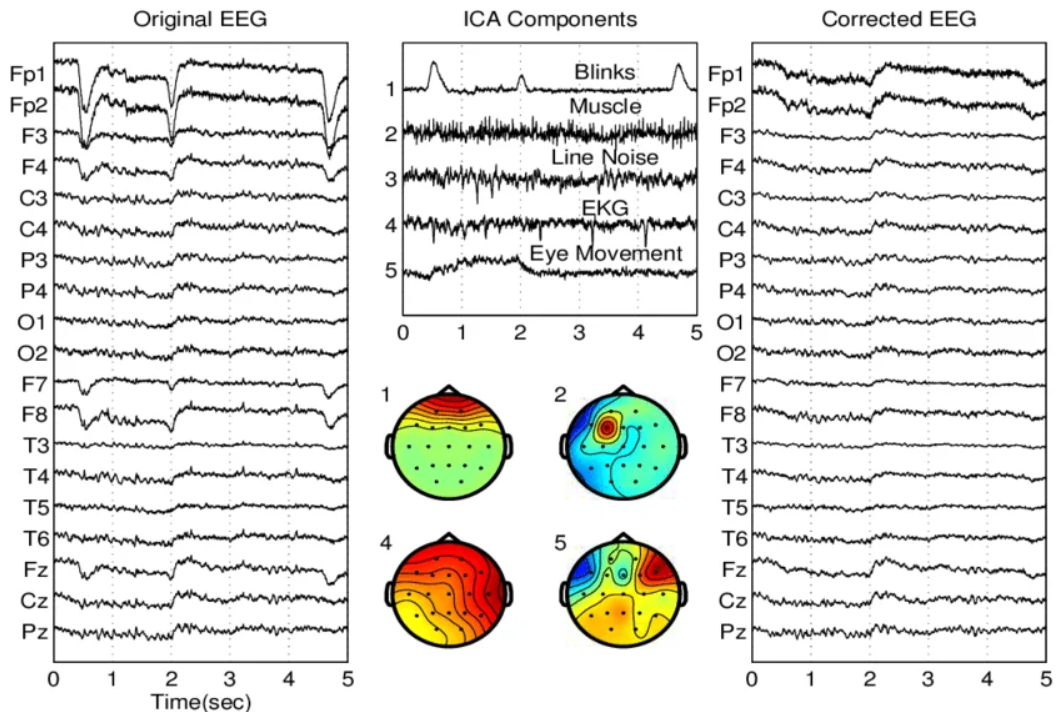
\includegraphics[width=\linewidth, ]{figuras/eeg_example.png}
    }
    \caption{Application of ICA in EEG preprocessing. ICA allows to separate physiological artifacts from the original EEG signal. \cite{jung_extended_1998}.}
    \label{fig:eeg_example}
\end{figure}

The success of ICA in EEG and other biomedical applications has motivated its use in EMG processing. However, these signals present specific challenges due to their amplitude variability and dependence on electrode position, muscle anatomy and activation patterns. For this reason, although BSS algorithms provide a useful approach for EMG source separation, its assumptions and limitations must be carefully considered before applying it to reinnervated muscle recordings.


\section{BSS Applied to EMG Decomposition}

In the context of EMG, the most relevant applications of blind source separation methods are found in high-density surface EMG decomposition. This is mainly because HD-sEMG recordings contain a large number of channels, which include spatial information about the original muscular activity. As a result, these recordings can be interpreted as mixtures of several physiological sources, making ICA and other separation algorithms suitable candidates for their decomposition.

ICA methods have been used to separate EMG recordings into components associated with different muscles or motor unit activity. By exploiting the statistical independence between sources, ICA can help isolate hidden components that are not directly observable from the raw electrode recordings. This is particularly useful when several muscles are active at the same time or when the activity recorded by one electrode is contaminated by nearby sources \cite{sato_crosstalk_2023,kim_frontiers_nodate,naik_applications_2011}.

However, applying separation algorithms to EMG is not straightforward. EMG sources are not always perfectly isolated and the recorded signals may be affected by noise, amplitude differences and temporal delays. These limitations become especially important in reinnervated muscle scenarios, where the target source may be weaker than the interfering donor-muscle activity. Therefore, although ICA provides a strong starting point for EMG decomposition, its assumptions and limitations must be carefully considered in the context of this thesis.

Even though separation algorithms have shown promising results in the applications
mentioned above, their use in asymmetric mixtures dominated by a stronger
interfering source has been less extensively studied. This is particularly relevant
for this thesis, where the objective is to recover a weak EMG target component
from that type of mixture.

\begin{figure}[H]
    \centering
    \makebox[\textwidth][c]{%
        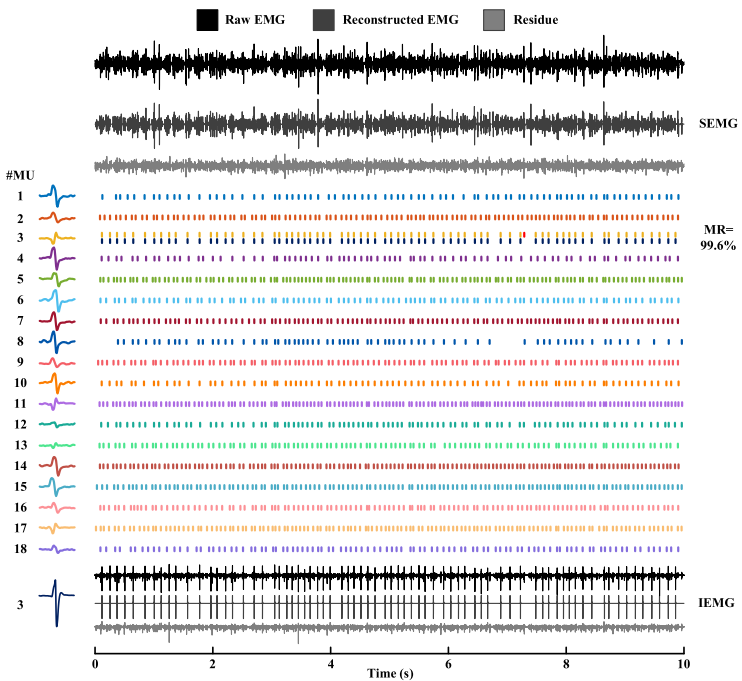
\includegraphics[width=\linewidth ]{figuras/sEMG_example.png}
    }
    \caption{High density surface EMG decomposition into motor unit activity using 2CFastICA\cite{chen_2cfastica_2024}.}
    \label{fig:sEMG_example}
\end{figure}

\clearpage
\section{Current Advances in Reinnervated EMG}

Recent research on reinnervated EMG has focused on improving the quality and
stability  of the signals generated by  nerve
interfaces. Techniques such as TMR, RPNIs and VDMTs have already been introduced
in Section~\ref{sec:motivation}. Therefore, this section focuses on how these
interfaces are currently evaluated from a signal processing perspective.

A common trend in the EMG literature is the use of recordings to assess
functional recovery after reinnervation. These recordings are used to evaluate
whether the reinnervated muscle produces detectable activation patterns, sufficient signal amplitude and reliable interpretation of the activity. In this sense, EMG is used as a control
signal as well as a tool to evaluate the success of the biological
interface.

\begin{figure}[H]
    \centering
    \makebox[\textwidth][c]{%
        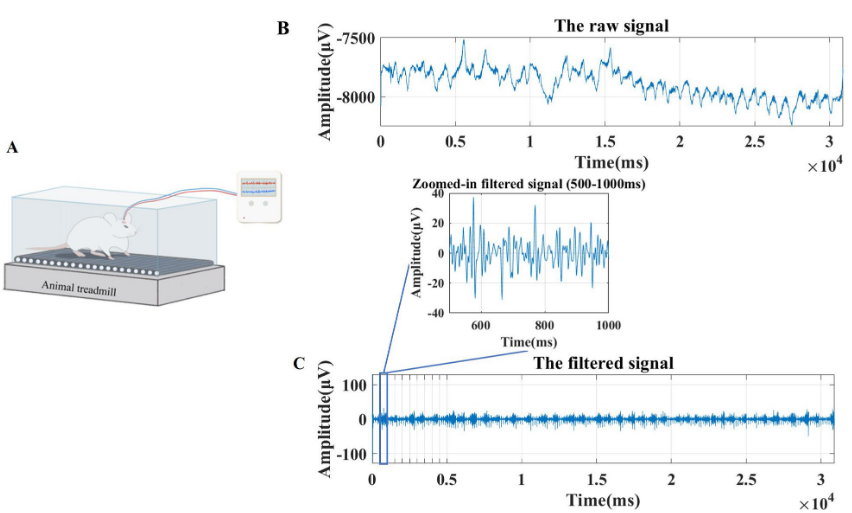
\includegraphics[width=\linewidth,height=8cm]{latex/anexos/Anexo B/figuras/EMG_rats.png}
    }
    \caption{Example study of reinnervated EMG assessment in animals. Current advances in reinnervated EMG are often first evaluated
    in experimental animal models \cite{tang_improving_2025}.}
    \label{fig:EMG_rats}
\end{figure}

Figure~\ref{fig:EMG_rats} illustrates this type of experimental evaluation, where
EMG measurements are used to assess nerve and muscle function after
reinnervation. Several current studies still rely on animal models before implementation in human prosthetic applications, which allows controlled analysis of
nerve regeneration, muscle response and signal evolution over time.

From a signal processing perspective, these studies show that reinnervated EMG is
a promising but complex source of information. Current work mainly focuses on
demonstrating functional recovery, signal detection and prosthetic control. However, fewer studies directly address how to separate a weak target
EMG component when it is mixed with stronger donor muscle
activity. This limitation connects the current advances in reinnervated EMG with
the research gap identified in the last section.
\clearpage
\section{Summary of source separation techniques in the literature}

The previous sections show that source separation methods have been applied in
different biomedical contexts, although often with objectives that differ from the
specific problem addressed in this thesis.

Classical ICA methods, including FastICA, Infomax and JADE, are mainly based on
statistical independence and have been widely used in EEG preprocessing, where
they allow the separation of neural activity from artifacts. Their success in
multichannel EEG has motivated their application to EMG, especially in
high-density recordings where the distribution of the electrodes provides
additional information about the muscular activity.

Other methods exploit different assumptions. SOBI uses delayed covariance
matrices and is more appropriate when the sources present different
temporal structures. Constrained ICA methods introduce prior information,
reference signals or correlation constraints to guide the separation towards
components with specific characteristics. Finally, regression  approaches are practical when a reliable interference reference is available.

Table~\ref{tab:literature_techniques} summarizes the main techniques found in the
literature, their typical application field and their relevance to the recovery
of weak EMG components.

\begin{table}[H]
\centering
\renewcommand{\arraystretch}{1.2}
\small
\begin{tabular}{p{3.2cm} p{4.2cm} p{5.2cm}}
\hline
\textbf{Technique} & \textbf{Application field} & \textbf{Main observation} \\
\hline

ICA / FastICA &
EEG preprocessing and EMG decomposition &
Commonly used for artifact removal and source decomposition when the mixture is approximately linear and instantaneous \cite{jung_extended_1998,naik_applications_2011}. \\

Infomax / JADE &
Biomedical BSS, especially EEG &
Alternative ICA implementations with similar assumptions \cite{kanna_advanced_2019}. \\

SOBI &
Signals with temporal structure &
Useful when sources have different temporal patterns, but less robust when EMG activations are temporally similar \cite{kalogiannis_reworked_2017}. \\

Constrained ICA / 2CFastICA &
HD-sEMG decomposition &
Improves decomposition when useful prior information or references can guide the separation \cite{chen_2cfastica_2024}. \\

Regression-based methods &
Interference reduction in biomedical signals &
Practical when a reliable reference of the interference is available, but sensitive to delay, noise and reference contamination \cite{gokcesu_adaptive_2019,jiang_removal_2019}. \\

\hline
\end{tabular}
\caption{Summary of source separation techniques reported in the literature.}
\label{tab:literature_techniques}
\end{table}

Overall, these methods have shown good results in EEG artifact removal and
HD-sEMG decomposition. However, few studies focus specifically on the recovery of
a weak EMG target source from an asymmetric mixture dominated by stronger muscle
interference. This limitation motivates the research gap addressed in the
following section.

\section{Research gap}


Previous studies have shown that BSS and semi-blind methods can be useful for biomedical signals, especially in EEG artifact removal and HD-sEMG decomposition \cite{jung_extended_1998,chen_2cfastica_2024}. However, most of these works focus on artifact removal or motor unit decomposition, rather than on the recovery of a weak EMG source masked by a stronger interfering muscle component.

This limitation is especially relevant in reinnervated EMG, where donor muscles may contaminate the target signal \cite{vu_regenerative_2020,tuffaha_vascularized_2020,tang_improving_2025}. In addition, standard separation methods assume instantaneous mixtures and
comparable source contributions, assumptions that may be weakened by noise,
source dominance and small temporal delays.

Therefore, this thesis addresses the gap between general EMG decomposition
methods and the recovery of weak target components in reinnervated muscle
recordings. In particular, it focuses on cases affected by stronger interference, additive
noise and possible temporal delays.